\documentclass{article}
    \author{杨铭\\5130379022}
    \title{计算机图形学 - 魁地奇桌球}
\usepackage{ctex}
\usepackage{graphicx}
\usepackage{color}
\usepackage{listings}
\usepackage{xcolor}
    \definecolor{gray}{rgb}{0.9,0.9,0.9}
\begin{document}
\lstset{numbers=left,
numberstyle=\tiny,
keywordstyle=\color{blue!70}, commentstyle=\color{red!50!green!50!blue!50},
frame=shadowbox,
rulesepcolor=\color{red!30!green!30!blue!30}
}
    \maketitle
    \renewcommand{\contentsname}{目\ \ 录}
    \tableofcontents
    \section{简述}
        \subsection{开发环境}
            \begin{description}
              \item[操作系统] windows7旗舰版
              \item[开发软件] Visual Studio 2015 community
              \item[模型制作] 3Ds MAX 2013
              \item[图形库] OpenGL4.4
              \item[CPU] Intel Xeon E3-1231v3 @3.4GHz
            \end{description}
            \paragraph{}使用了opengl的核心库和相关辅助库gl、glu、glut、glew、glaux,使用3ds Max制作场景和地形模型
        \subsection{完成功能}
            \paragraph{}
            在第二次迭代的基础上,完成了以下功能:
            \begin{itemize}
              \item 读取obj模型文件并进行场景和地形的模型制作与渲染
              \item 完善光照效果,追加一个紧跟母球的聚光灯
              \item 实现简单版本的3D物理引擎
              \item 使用perlin噪声为小球生成随机纹理
              \item 天空盒
              \item 完善视角控制
              \item 粒子特效
            \end{itemize}
    \section{设计说明}
        \subsection{程序结构}
            \paragraph{}主程序为QuidditchApp.exe,跟res文件夹放在统计目录下可以直接运行。
            \paragraph{程序结构}
                程序包含:\\
                \begin{itemize}
                  \item Club
                  \item Flag
                  \item Hill
                  \item Object
                  \item Orb
                  \item Particle、ParticleSystem
                  \item Skybox
                  \item Table
                  \item Terrain
                \end{itemize}
                等图形类,以及
                \begin{itemize}
                  \item Controller
                  \item Camera
                  \item Texture
                  \item Physical
                  \item Point3d、Vector3D
                \end{itemize}
                等辅助类,其中\textbf{Controller}负责交互控制、\textbf{Camera}负责视角控制、\textbf{Texture}负责保存perlin噪声生成的纹理、\textbf{Physical}是物理引擎、\textbf{Point3D}和\textbf{Vector3D}为三维点和向量辅助类
        \subsection{文件路径说明}
            \paragraph{}
                "res"文件夹必须放在主程序同级目录下,否则无法正常加载.obj文件和纹理
    \section{实现过程}
        \subsection{读取obj模型文件和绘制}
            \paragraph{}
                .obj是一种通用的3D模型文件格式。由Alias|Wavefront公司为3D建模和动画软件"Advanced Visualizer"开发的一种标准,适合用于3D软件模型之间的互导。.obj文件一般分为4个部分,分别记录定点坐标、法向量坐标、纹理映射坐标和面片连接方式  
                本次迭代实现了对obj的读取和绘制,并且使用了VAO(Vertex Array Object)的加速绘制方法,使得对于40000个点,上万个面片的绘制也能做到快速。但是较多个模型的场景会导致.obj文件的变大,在读文件时速度较慢。
                \begin{lstlisting}[language={[ANSI]C}]
for (std::list<SubMesh*>::iterator i = children.begin(); 
    i != children.end(); i++) 
{
  Material mt = material_map[(*i)->mtName];
  SetMaterial(GL_FRONT_AND_BACK, GL_AMBIENT, mt.ka);
  SetMaterial(GL_FRONT_AND_BACK, GL_DIFFUSE, mt.kd);
  SetMaterial(GL_FRONT_AND_BACK, GL_SPECULAR, mt.ks);
  glBindTexture(GL_TEXTURE_2D, mt.kd_texid);
  glVertexPointer(3, GL_FLOAT, 0, (*i)->ptBuffer);
  glTexCoordPointer(2, GL_FLOAT, 0, (*i)->uvBuffer);
  glNormalPointer(GL_FLOAT, 0, (*i)->nmBuffer);
  glDrawArrays(GL_TRIANGLES, 0, (*i)->vNum);
}
                \end{lstlisting}
            \paragraph{}我自己绘制了地形和城墙,坦克模型从网上下载,纯属观赏(使用了一个立方体碰撞包围盒覆盖它)
        \subsection{光照效果}
            \paragraph{聚光灯}对OpenGL里的光照设置GL\_SPOT\_DIRECTION,这个光源会被认为是聚光灯。通过对它位置、聚光程度和收敛角的设置,可以达到追踪母球的效果
            \begin{lstlisting}[language={[ANSI]C}]
glEnable(GL_LIGHT1);
glLightfv(GL_LIGHT1, GL_POSITION, light1_position);
glLightfv(GL_LIGHT1, GL_AMBIENT, light1_ambient);
glLightfv(GL_LIGHT1, GL_DIFFUSE, light1_diffuse);
glLightfv(GL_LIGHT1, GL_SPECULAR, light1_specular);
glLightf(GL_LIGHT1, GL_SPOT_CUTOFF, 24.0);
glLightfv(GL_LIGHT1, GL_SPOT_DIRECTION, light1_spotdir);
glLightf(GL_LIGHT1, GL_SPOT_EXPONENT, 1.0); 
            \end{lstlisting}
            \paragraph{}
                上面的代码设置了一个初始位置在母球上方的光源,并指明它的方向垂直指向地面,也就是母球。然后设置了它的收敛角度和汇聚强度
            \paragraph{}
                需要注意的是光照的位置和方向会受到视角矩阵的影响,需要每一帧重新设置它们
            \begin{lstlisting}[language={[ANSI]C}]
void setlights(void)
{
	Point3D mPos = crashManager->getMPos();
	light1_position[0] = mPos.x;
	light1_position[1] = mPos.y;
	glLightfv(GL_LIGHT0, GL_POSITION, light0_position);
	glLightfv(GL_LIGHT1, GL_POSITION, light1_position);
	glLightfv(GL_LIGHT1, GL_SPOT_DIRECTION, light1_spotdir);
}
            \end{lstlisting}
            \paragraph{}
                最后添加了交互控制,按'b'键可以开关聚光灯
        \subsection{实现简单版本的3D物理引擎}
            \paragraph{}
                由于地形是读取的obj文件,为了方便代码的编写和计算,我在设计地形时做了简化,使得地形被剖分的点的坐标均为整数,并且所有坐标上的点都均匀分布。
                \begin{figure}[bhtp]
                    \begin{minipage}[bhtp!]{1\linewidth}\centering
                    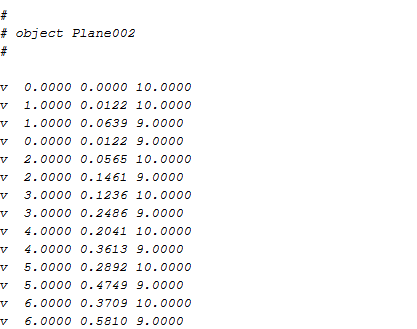
\includegraphics[width=9cm]{v.png}
                    \caption{地形obj格式}\label{1-a}
                    \end{minipage}
                \end{figure}
            \paragraph{}
                这样我们就可以构建一个地形的高度表,对应\textbf{Hill}类中的heightDiagram。一个高度表是一个二维数组,它的两个维度分别为地形横向的点数和纵向的点数,而模型保证了这些点均匀分布,就可以简单的根据点的坐标映射到高度表的坐标中,从而根据点的x、y轴坐标直接索引到点所在的高度
            \begin{lstlisting}[language={[ANSI]C}]
float Hill::getHeight(float x, float y)
{
	if (heightDiagram!=NULL)
	{
		// round to nearest integer
		int px = int(x);
		int py = int(y);
		float frcx = x - px;
		float frcy = y - py;
		if (frcx >= 0.5)
			px += 1;
		if (frcy >= 0.5)
			py += 1;
		py += 10;
		return heightDiagram[py][px];
	}
	else
	{
		return 0.0f;
	}
}
            \end{lstlisting}
            \paragraph{}
                这样我们可以实现让小球永远贴着地表做三维运动。在每一帧里判断有没有小球落在了“高低”的范围内,如果有,则根据它的坐标,找到离小球最近的3个“高地”的点,接着通过线性插值的方式计算出小球的高度。
            \paragraph{}
                当然这种实现并不是真实的物理模型,只是对真实世界的一种简化。
        \subsection{使用perlin噪声为小球生成随机纹理}
            \paragraph{Perlin噪声}
                使得随机变得“有序”的一种算法或者说思想。perlin噪声使用插值和多频率叠加等方式使得随机生成的点被连接成为光环的曲线,然后通过曲线中所有的点映射到任意大的范围内生成数据。
            \paragraph{}
                我使用了一个二维的噪声生成器,然后通过cos插值和3个频率的叠加生成了最终的噪声数据。并把这个数据映射到0-255的范围内作为灰度值来使用
            \begin{lstlisting}[language={[ANSI]C}]
Texture* genTexture(int seed)
{
  Texture *tex = new Texture();
  tex->sizeX = TEX_X;
  tex->sizeY = TEX_Y;
  tex->data = new unsigned char[TEX_X*TEX_Y * 3];
  for (int i = 0; i < TEX_Y; i++)
  {
  	for (int j = 0; j < TEX_X; j++)
	{
	  unsigned char value = LEVEL*perlinNoise(float(j+seed)
                             / 64.0f, float(i+seed) / 64.0f);
	  tex->data[(j + i*TEX_X) * 3]     = value;
	  tex->data[(j + i*TEX_X) * 3 + 1] = value;
	  tex->data[(j + i*TEX_X) * 3 + 2] = value;
	}
  }
  return tex;
}
            \end{lstlisting}
        \subsection{天空盒}
            \paragraph{}使用Terrgen工具生成一张全景图,然后使用CubeTheShpere工具将其分解为6张图片,分别对应天空盒的前后左右上下六个方向。然后在场景中绘制一个大的立方体,并按照正确的顺序将
            上面生成的图片贴在对应的立方体面上即可完成
                        \begin{lstlisting}[language={[ANSI]C}]
void Skybox::render()
{
  glPushMatrix();

  glTranslatef(x, y, z);
  glRotatef(90, 1.0, 0, 0);
  glEnable(GL_TEXTURE_2D);
  glDisable(GL_LIGHTING);

  glTexEnvf(GL_TEXTURE_ENV, GL_TEXTURE_ENV_MODE, GL_DECAL);
  glBindTexture(GL_TEXTURE_2D, DOWN_TEX);

  glBegin(GL_QUADS);
	glTexCoord2f(1.0f, 1.0f); 
    glVertex3f(-EMAX,EMAX,-EMAX);	
	glTexCoord2f(0.0f, 1.0f); 
    glVertex3f(-EMAX,EMAX,EMAX);	
	glTexCoord2f(1.0f, 0.0f); 
    glVertex3f(EMAX,EMAX,EMAX);  	
	glTexCoord2f(0.0f, 0.0f); 
    glVertex3f(EMAX,EMAX,-EMAX);	
  glEnd();
  ...
            \end{lstlisting}
        \subsection{完善视角控制}
            \paragraph{}
            增加了横向和远近方向上的控制。使得它不再像以前那样蛋疼了(虽然依旧比较蛋疼)
        \subsection{粒子特效}
            \paragraph{原理}
            粒子特效,即使用大量小的物体做随机运动来模拟自然界中粒子的效果。进一步可以控制粒子运动的趋势,改变粒子的颜色,实现粒子的碰撞,增加粒子运动时的动态模糊等增加真实感和画面的绚丽程度
            \paragraph{}
            为了实现粒子效果,我定了\textbf{Particle} 类,作为一个单独的粒子,再定义一个控制粒子的类\textbf{ParticleSystem},作为所有粒子系统的基类。独特的粒子继承自\textbf{ParticleSystem},但是对其一些属性或者绘制方式做了修改
            \begin{lstlisting}[language={[ANSI]C}]
class Particle
{
public:
  Particle() {};
  Vector3D position;
  Vector3D velocity;
  Vector3D acceleration;
  Color color;
  float age;
  float life;
  float size;
  bool active;
};
            \end{lstlisting}
            \paragraph{Spark}
            Spark为球与球碰撞产生的火花粒子特效,继承自\textbf{ParticleSystem},它使用了一张半透明的贴图,并且使用彩虹表中的随机颜色对纹理进行混合模式的上色。对粒子应用较快的四散的初速度和恒定的重力加速度,模拟爆炸火花的效果。
            \begin{lstlisting}[language={[ANSI]C}]
void Spark::render()
{
  if (isActive())
  {
	glEnable(GL_TEXTURE_2D);	
	glDisable(GL_LIGHTING);
	glDisable(GL_DEPTH_TEST);
	glBindTexture(GL_TEXTURE_2D, TEX_PARTICLE);
	glEnable(GL_BLEND);
	glBlendFunc(GL_SRC_ALPHA, GL_ONE);
	glTexEnvf(GL_TEXTURE_ENV, GL_TEXTURE_ENV_MODE, GL_MODULATE);
	for (vector<Particle*>::iterator iter = particles.begin(); 
         iter != particles.end(); iter++)
	{
	  if ((*iter)->active)
	  {
		float x = (*iter)->position.x;
		float y = (*iter)->position.y;
		float z = (*iter)->position.z;
		Color color = (*iter)->color;
		float alpha = 1.0 - (*iter)->age / (*iter)->life;
		glColor4f(color.r, color.g, color.b, alpha);
		float sz = 0.5;
		glPushMatrix();
		glBegin(GL_TRIANGLE_STRIP);
		glTexCoord2d(1, 1); 
        glVertex3f(x + sz / 2, y + sz / 2, z);
		glTexCoord2d(0, 1); 
        glVertex3f(x - sz / 2, y + sz / 2, z);
		glTexCoord2d(1, 0); 
        glVertex3f(x + sz / 2, y - sz / 2, z);
		glTexCoord2d(0, 0); 
        glVertex3f(x - sz / 2, y - sz / 2, z);
		glEnd();
		glPopMatrix();
	  }
	}
	glEnable(GL_LIGHTING);
	glDisable(GL_TEXTURE_2D);
	glEnable(GL_DEPTH_TEST);
	glDisable(GL_BLEND);
  }	
}
            \end{lstlisting}
            \paragraph{}
    \section{效果展示}
        \paragraph{}
            由于模型文件较大(8.89M),导致每次开始执行要浪费大量时间在读文件上,而且多个面片在对光照的映射处理导致帧数也有一定的降低
            \begin{figure}[bhtp]
                    \begin{minipage}[bhtp!]{1\linewidth}\centering
                    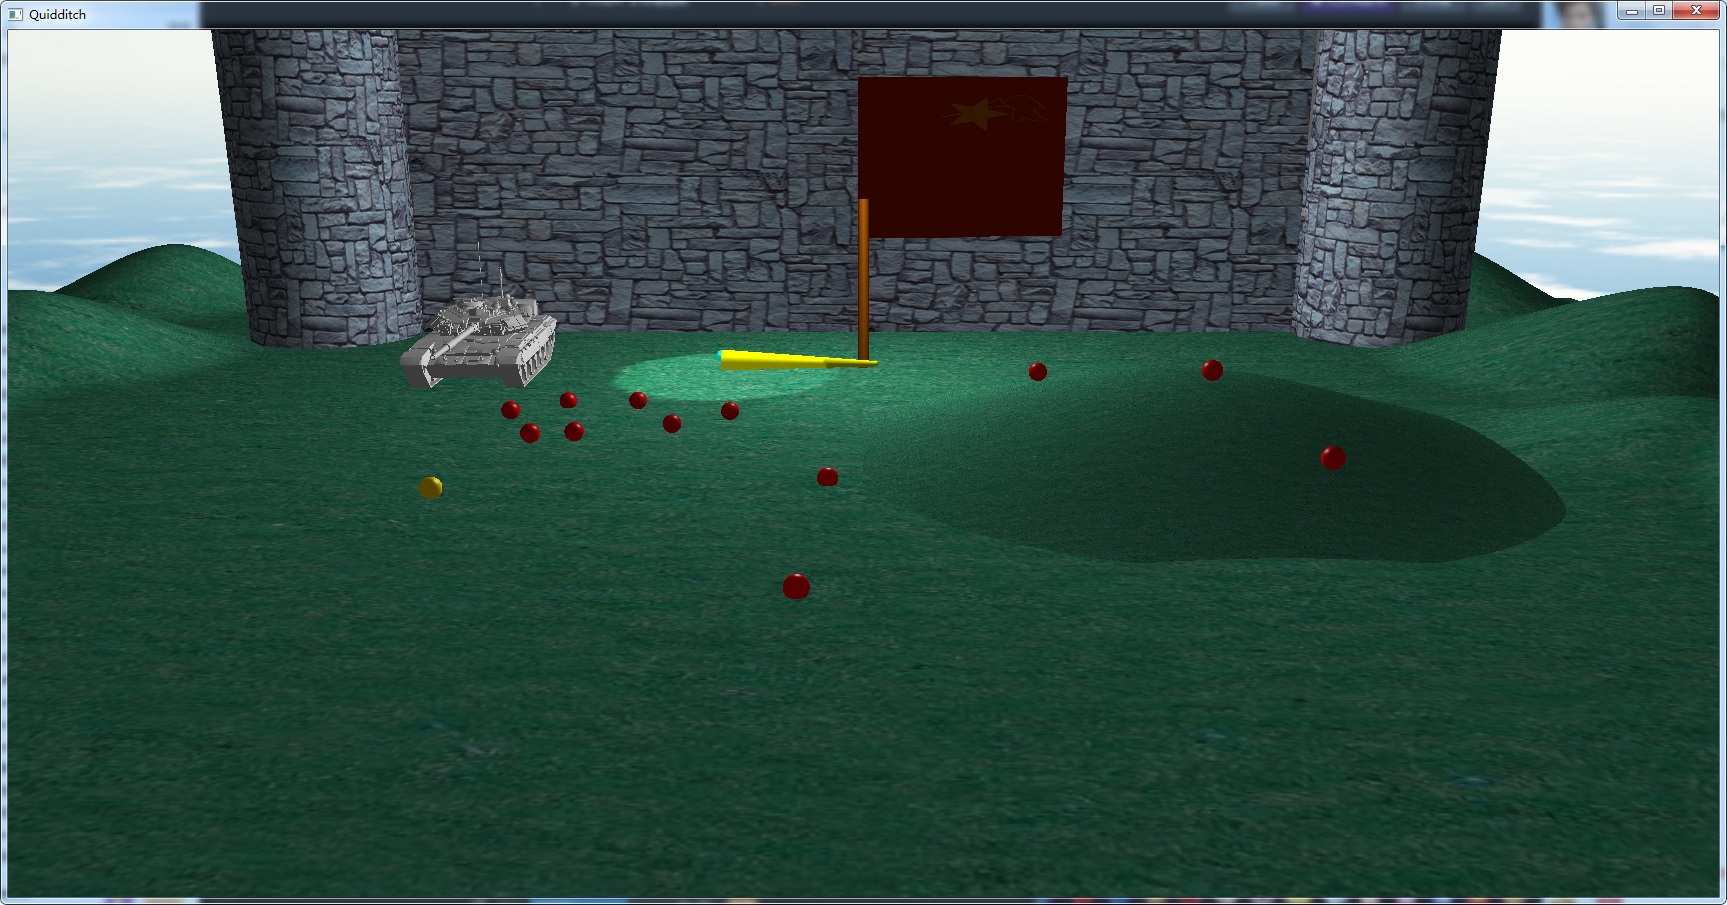
\includegraphics[width=12cm]{result.png}
                    \caption{结果图}\label{2-a}
                    \end{minipage}
                \end{figure}

\end{document}
